\chapter{Bandt-Pompe Symbolization: Concepts and definitions}\label{chapter:BP}

Dynamic systems describe the relationship in time of a point in a geometric space.
Thus, the study of time series assists in the analysis of the dynamics of its generating processes.
Whether a scalar time series collected through the observation of natural phenomena or obtained through synthetic simulations, its values will be the result of a function formed by its majority of unobserved and measured variables.
Thus, an important research question in data analysis has been:
\begin{quote}
    Given a system and a sample resulting from it whose evolution can be tracked over time, how much information is encoded in this observable about the dynamics of the underlying system and the variables that characterize them?
\end{quote}
Traditionally, the study of time series is carried out under two lines of study, in the domains of time and frequency~\citep{BrockwellDavis91}.
However, both approaches directly use the data resulting from the observational process, which are sensitive to noise and contamination effects.
The approach to the use of non-parametric methods appears in the literature as a way to prevent such effects from compromising the analyzes.

To make good inferences in data analysis studies, it is expected that the proposed approach meets the following requirements:
\begin{itemize}
    \item Be simple, fast and transparent;
    \item Make little or no assumptions about the underlying process; and
    \item Be resilient towards outliers.
\end{itemize}
When analyzing classic probabilistic techniques, we found that they cannot obtain good results without assuming characteristic properties of the data, such as the shape of the probability distribution of the samples.
On the other hand, proposals based on machine learning do not mean to guarantee the required simplicity and transparency, as they do not provide a clear view of the observed characteristics~\citep{bandt2019small}.

The \num{1820} citations received by the seminal paper appeared in \num{684} journals indexed by the Web of Science.
These journals belong to \num{127} categories, spanning from Multidisciplinary Physics (\SI{24}{\percent} of the publications) to Zoology (only one of the of citing articles).
There are \num{17} citing articles from journals that belong to the Statistics \& Probability category.
Five of these articles appeared in \textit{Stochastic Environmental Research and Risk Assessment}, 
two in the \textit{Journal of Time Series Analysis}, 
and each of the remaining ten appeared in a different journal.
Most of these articles relate successful applications of the Bandt and Pompe methodology, except \cite{OrdinalPatternProbabilities} that obtained the sample entropy's properties under zero-mean Gaussian processes.
It is also noteworthy that, in this category of publications, \cite{DistributionsofOrderPatternsofIntervalMaps} provided a formal and more general proof of the structure of the boundary of the $H\times C$ manifold than that obtained by \cite{martin2006generalized}.
The lack of attention that the Bandt and Pompe approach has received by the Probability \& Statistics community confirms that it is a fertile research avenue waiting to explore.

In this context, the analysis of ordinal patterns coupled with the use of information theory descriptors, in addition to meeting the requirements above, has been able to detect causal information related to the unobserved variables that control the system, in addition to identifying chaotic components, visualization and characterization of different dynamic regimes, among other applications.

\section{Ordinal Patterns Representation}\label{sub:ordinalPatterns}

\cite{Bandt2002Permutation} introduced the representation of time series by ordinal patterns as a transformation resistant to noise, and invariant to nonlinear monotonic transformations.
Let ${\mathcal X} \equiv \{x_t\}_{t=1}^{T}$ be a real valued time series of length $T$, without ties. 
As stated by \cite{Bandt2002Permutation} in their seminal work:  
\begin{quote}
``If the $\{x_t\}_{t=1}^{T}$ attain infinitely many values, it is common to replace them by a symbol sequence 
$\Pi \equiv \{\pi_j\}$ with finitely many symbols, and calculate source entropy from it".
\end{quote}
Also, as stressed by these authors, 
\begin{quote}
``The corresponding symbol sequence must come 
naturally from the $\{x_t\}_{t=1}^{T}$ without former model assumptions".
\end{quote}

Let ${\mathfrak A}_{D}$ (with $D \geq 2$ and $D \in {\Bbb N}$) be the symmetric group of order $D!$ formed by all 
possible permutation of order $D$, and the symbol component vector 
${\bm \pi}^{(D)} = (\pi_1, \pi_2, \dots, \pi_D)$ so every element ${\bm \pi}^{(D)}$ is unique 
($\pi_j \neq \pi_k$ for every $j \neq k$). 
Consider for the time series ${\mathcal X} \equiv \{x_t\}_{t=1}^{T}$ its time delay embedding representation,
with embedding dimension $D \geq 2$ and time delay $\tau \geq 1$ ($\tau \in {\Bbb N}$, also called ``embedding time,'' ``time delay'', or ``delay''):
\begin{equation} 
\label{SAR:eq:time-delay}
{\mathbf X}^{(D,\tau)}_t =( x_t,x_{t+\tau},\dots,x_{t+(D-1)\tau} ) ,
\end{equation} 
for $t = 1,2,\dots,N$ with $N = T-(D-1) \tau$.
Then the vector ${\mathbf X}^{(D,\tau)}_t$ can be mapped to a symbol vector ${ \widetilde{\bm \pi}}_t^D \in {\mathfrak A}_{D}$. 
This mapping is such that preserves the desired relation between the elements 
$x_t  \in {\mathbf X}^{(D,\tau)}_t$, and all $t \in \{1,\dots,T-(D-1)\tau\}$ that share this pattern (also called ``motif'') are mapped to the same 
${\widetilde{\bm \pi}}_t^{D}$.

We define the mapping ${\mathbf X}_t^{(D,\tau)} \mapsto {\widetilde{\pi}}_t^{D}$ by ordering the observations $x_t \in {\mathbf X}_t^{(D,\tau)}$ in increasing order.
Consider the time series:
\begin{equation}
    \mathcal X = (1.8, 1.2, 3.2, 4.8, 4.2, 4.5, 2.3, 3.7, 1.2, 0.5)
    \label{eq:series}
\end{equation}
depicted in Fig.~\ref{SAR:Fig:IntroBP}.
Assume we are using patterns of length $D=5$ with unitary time lag $\tau=1$.
The code associated to $\mathbf X_{3}^{(5,1)}=(x_3,\dots,x_7)=(3.2, 4.8, 4.2, 4.5, 2.3)$, shown in black, is formed by the indexes in $\bm\pi_3^{5}=(1,2,3,4,5)$ which sort the elements of $\mathbf X_{3}^{(5,1)}$ in increasing order: $51342$.
With this, $\widetilde{\pi}_3^{5} = 51342$, and we increase the counting related to this motif in the histogram of all possible patterns of size $D=5$.

The dash-dot line in Fig.~\ref{SAR:Fig:IntroBP} illustrates $\mathbf X_{1}^{(5,2)}$, i.e. the sequence of length $D=5$ starting at $x_1$ with lag $\tau=2$.
In this case, $\mathbf X_{1}^{(5,2)}= (1.8, 3.2, 4.2, 2.3, 1.2)$, and the corresponding motif is $\widetilde{\pi}_1^{5}=51423$.

\begin{figure}
	\centering
	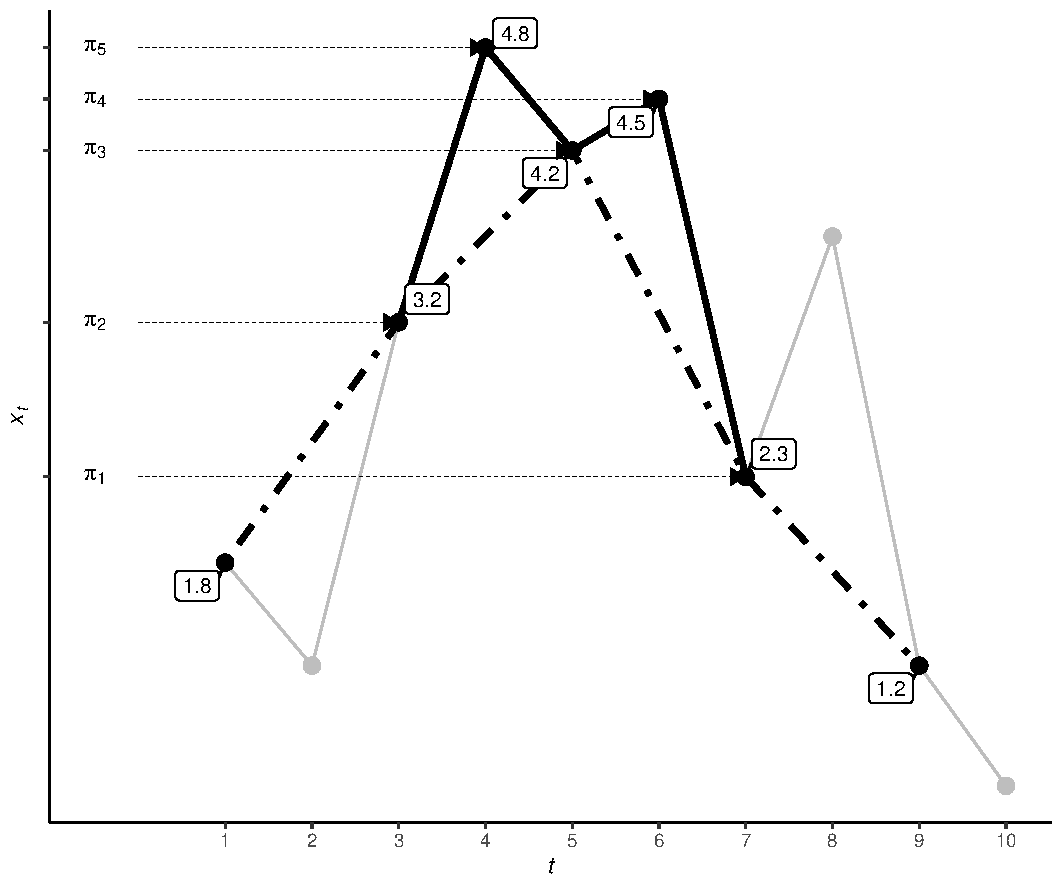
\includegraphics[width=.9\linewidth]{Figures/IntroBP.pdf}
	\caption{Illustration of the Bandt and Pompe coding\label{SAR:Fig:IntroBP}. Here the gray line represents the analyzed sequence $\mathcal X = (1.8, 1.2, 3.2, 4.8, 4.2, 4.5, 2.3, 3.7, 1.2, 0.5)$, the sequence illustrated by the dotted line shows the path taken when applying $\tau = 2$, and the sequence illustrated by the black line shows the elements of the pattern $\mathbf X_{1}^{(5,2)}= (1.8, 3.2, 4.2, 2.3, 1.2)$.}
\end{figure}

The classic approach to calculating the probability distribution of ordinal patterns is through the frequency histogram.
Denote $\Pi$ the sequence of symbols obtained by a given series $\mathbf{X}_t^{(D,\tau)}$.
The Bandt-Pompe probability distribution is the relative frequency of symbols in the series against the $D!$ possible patterns $\{\widetilde\pi_t^D \}_{t = 1}^{D!}$:
\begin{equation}
p(\widetilde\pi_t^D) = \frac{\#\left \{\mathbf{X}_t^{(D,\tau)} \text{ is of type } \widetilde\pi_t^D\right \}}{T- (D-1)\tau},  
\end{equation}
where  $t\in \{1, \dots, T-(D-1)\tau\}$.
These probabilities meet the conditions $p(\widetilde\pi_t^D) \ge 0$ and  $\sum_{i=1}^{D!} p(\widetilde\pi_t^D) = 1$, and are invariant before monotonic transformations of the time series values.
For example, the presence of $\alpha$ multiplicative noise in ${\mathcal X}$ does not change the results of the patterns produced.

In the literature, there are two ways to perform the mapping ${\mathbf X}_t^{(D, \tau)} \mapsto {\mathbf \pi}_t^{D}$ in the symbolization of Bandt-Pompe:~(i) Sorting the positions of the elements $x_t \in {\mathbf X}_t^{(D, \tau)}$ in chronological order (Permutation of Classification), and~(ii) Sorting the time indexes of the elements $x_t \in {\mathbf X}_t^{(D, \tau)}$ (Chronological Index Permutation).

\subsection{Rank Permutation Mapping}\label{sub:rankPermutation}

For an arbitrary $t$, the vector of real values $\mathcal{X}^{(D, \tau)}_t = (x_t, x_{t + 1}, \dots, x_{t + D - 1})$ with time delay $\tau \geq 1$ $(\tau \in \mathbb{Z})$, and embedding dimension $D \geq 2$ $(D \in \mathbb{Z})$ are mapped to the vector symbol $\bm \pi^D = (\bm R[x_t], \bm R[x_{t + 1}], \dots, \bm R[x_{t + D - 1}]) \in {\mathfrak A}_{D}$ formed by the rank of its components, defined as the following function:

\begin{equation}
    R[x_{t + n}] = \sum^{D - 1}_ {k = 0} \mathds{1} (x_{t + k} \leq x_{t + n}) \text{ for } n = 0, \dots, D - 1
\end{equation}
where $x_{t+n} \in X^{(D, \tau)}_t$, $1 \leq R(x_{t+n}) \leq D$, and $\mathds{1}$ is the indicator function: $\mathds{1}(Z) = 1$ if $Z$ is true and $0$ otherwise.  
So the maximum and minimum values of rank are $R(\min(x_{t+k})) = 1$ and $R(\max(x_{t+k})) = D$.
The complete alphabet is all the possible permutation of the ranks.
Examples of its application can be seen in~\cite{riedl2013practical} and~\cite{bandt2007order}.

For example, let us take the series~\ref{eq:series}, time delay $\tau = 1$ and embedding dimension $D = 3$, the eight vectors and their corresponding patterns obtained by rank permutation mapping are:

\begin{center}
    \scalebox{.8}{
    \begin{minipage}[b]{0.5\textwidth}
        \raggedright
        \begin{equation*}
            \bm X^{(3, 1)}_1 = (1.8, 1.2, 3.2) \mapsto (2,1,3),
        \end{equation*}
        \begin{equation*}
            \bm X^{(3, 1)}_2 = (1.2, 3.2, 4.8) \mapsto (1,2,3),
        \end{equation*}
        \begin{equation*}
            \bm X^{(3, 1)}_3 = (3.2, 4.8, 4.2) \mapsto (1,3,2),
        \end{equation*}
        \begin{equation*}
            \bm X^{(3, 1)}_4 = (4.8, 4.2, 4.5) \mapsto (3,1,2),
        \end{equation*}
    \end{minipage}
    \begin{minipage}[b]{0.5\textwidth}
        \raggedright
        \begin{equation*}
            \bm X^{(3, 1)}_5 = (4.2, 4.5, 2.3) \mapsto (2,3,1),
        \end{equation*}
        \begin{equation*}
            \bm X^{(3, 1)}_6 = (4.5, 2.3, 3.7) \mapsto (3,1,2),
        \end{equation*}
        \begin{equation*}
            \bm X^{(3, 1)}_7 = (2.3, 3.7, 1.2) \mapsto (2,3,1),
        \end{equation*}
        \begin{equation*}
            \bm X^{(3, 1)}_8 = (3.7, 1.2, 0.5) \mapsto (3,2,1),
        \end{equation*}
    \end{minipage}}
\end{center}

In Fig.~\ref{fig:Rank}, we present an illustrative drawing of this mapping for all alternatives when we have $D = 3$.
As we can see, the vertical axis indexes are fixed and the resulting pattern is obtained through the time axis labels in chronological order.

\begin{figure}
    \centering
    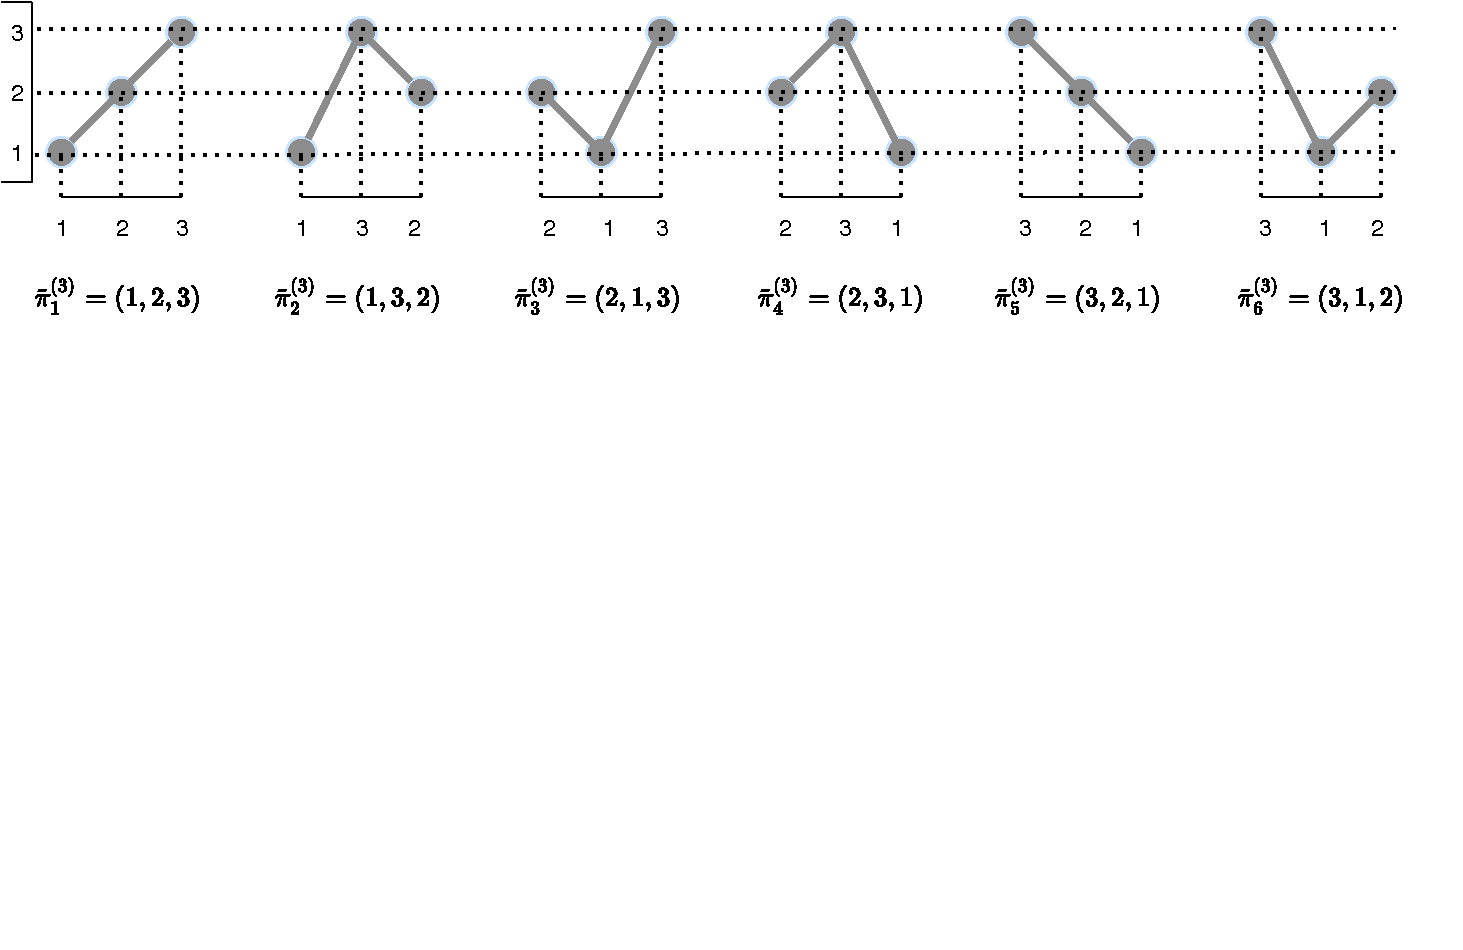
\includegraphics[width=\linewidth]{Figures/rank.pdf}
    \caption{\textbf{Rank permutation mapping:} The complete alphabet for $D = 3$ of the rank mapping technique obtained by permuting all possible ranks.}
    \label{fig:Rank}
\end{figure}

\subsection{Chronological Index Permutation Mapping}\label{sub:chronological}

Again, for an arbitrary $t$, the vector of real values $\mathcal{X}^{(D, \tau)}_t = (x_t, x_{t + 1}, \dots, x_{t + D - 1})$ with time delay $\tau \geq 1$ $(\tau \in \mathbb{Z})$, and embedding dimension $D \geq 2$ $(D \in \mathbb{Z})$ are mapped to the vector symbol $\bm \pi^D = (\bm i_1, \bm i_2, \dots, \bm i_D) \in {\mathfrak A}_{D}$ formed by  the time indexes ordered according to their amplitudes. 
So, the sequence must comply $x_{t+i_1} < x_{t+i_2} < \dots < x_{t+i_D}$. 
Examples of its application can be seen in~\cite{Bandt2002Permutation}, ~\cite{DistinguishingNoiseFromChaos},~\cite{parlitz2012classifying}, and~\cite{bian2012modified}.

For example, let us take the series~\ref{eq:series}, time delay $\tau = 1$ and embedding dimension $D = 3$, the eight vectors and their corresponding patterns obtained by rank permutation mapping are:

\begin{center}
    \scalebox{.8}{
    \begin{minipage}[b]{0.5\textwidth}
        \raggedright
        \begin{equation*}
            \bm X^{(3, 1)}_1 = (1.8, 1.2, 3.2) \mapsto (2,1,3),
        \end{equation*}
        \begin{equation*}
            \bm X^{(3, 1)}_2 = (1.2, 3.2, 4.8) \mapsto (1,2,3),
        \end{equation*}
        \begin{equation*}
            \bm X^{(3, 1)}_3 = (3.2, 4.8, 4.2) \mapsto (1,3,2),
        \end{equation*}
        \begin{equation*}
            \bm X^{(3, 1)}_4 = (4.8, 4.2, 4.5) \mapsto (2,3,1),
        \end{equation*}
    \end{minipage}
    \begin{minipage}[b]{0.5\textwidth}
        \raggedright
        \begin{equation*}
            \bm X^{(3, 1)}_5 = (4.2, 4.5, 2.3) \mapsto (3,1,2),
        \end{equation*}
        \begin{equation*}
            \bm X^{(3, 1)}_6 = (4.5, 2.3, 3.7) \mapsto (2,3,1),
        \end{equation*}
        \begin{equation*}
            \bm X^{(3, 1)}_7 = (2.3, 3.7, 1.2) \mapsto (3,1,2),
        \end{equation*}
        \begin{equation*}
            \bm X^{(3, 1)}_8 = (3.7, 1.2, 0.5) \mapsto (3,2,1),
        \end{equation*}
    \end{minipage}}
\end{center}

In Fig.~\ref{fig:Chronological}, we present an illustrative drawing of this mapping for all alternatives when we have $D = 3$.
In this mapping, the time indexes are fixed in chronological order.
The patterns are chosen by the vertical axis labels in the increasing direction of the amplitude.

\begin{figure}
    \centering
    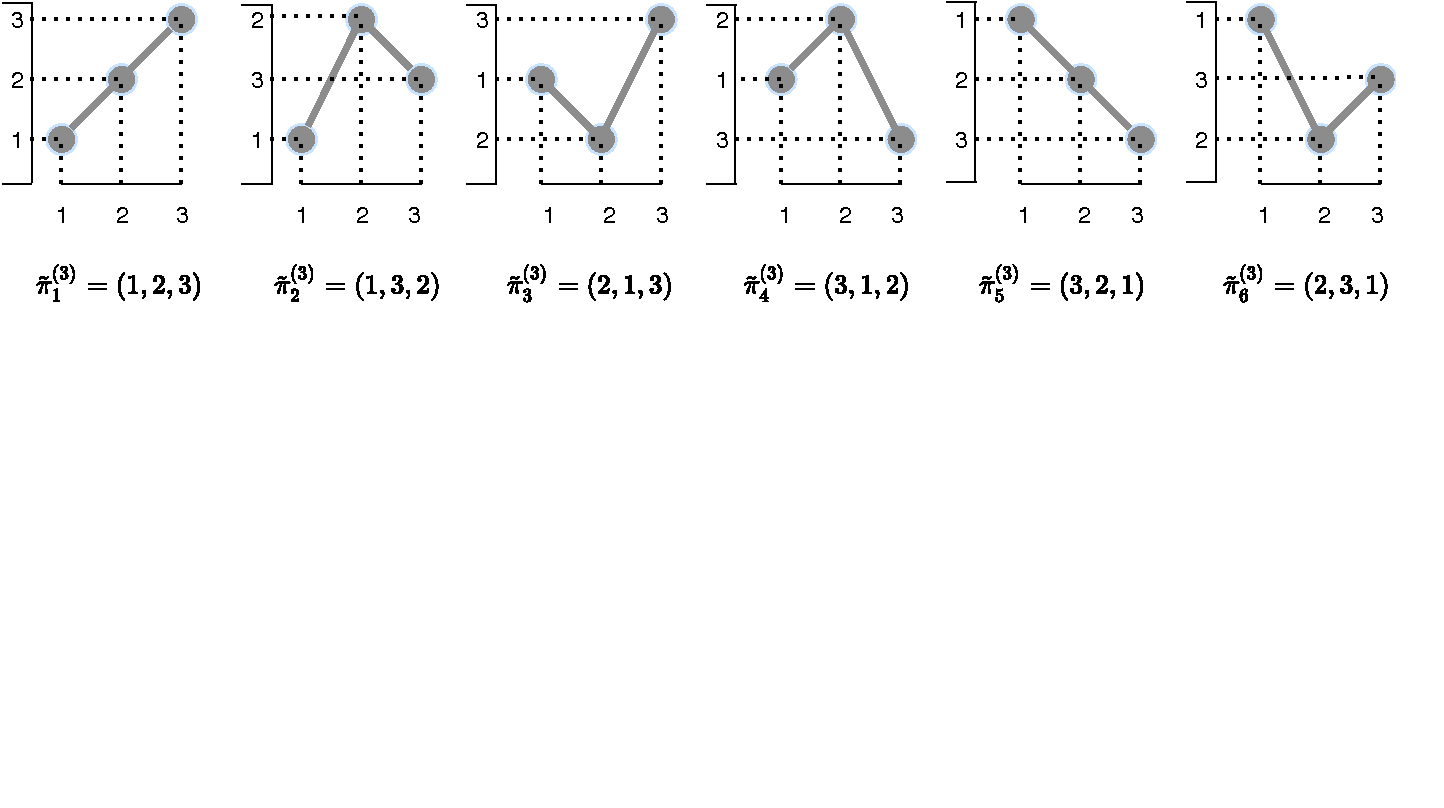
\includegraphics[width=\linewidth]{Figures/Chronological.pdf}
    \caption{\textbf{Chronological index permutation mapping:} The complete alphabet for $D = 3$ of the chronological mapping technique obtained by permuting all of its indexes.}
    \label{fig:Chronological}
\end{figure}

\section{Ordinal Patterns Transition Graphs}\label{sub:OPTG}

Alternatively, given the sequence of ordinal patterns $\Pi$ one may form an oriented graph with the transitions from $\widetilde\pi_t^D$ to $\widetilde\pi_{t+1}^D$. 
The Ordinal Pattern Transition Graph ${G} = ({V}, {E})$ 
represents the transitions between two consecutive ordinal patterns over time $t$.
The vertices are the $D!$ possible patterns for an embedding dimension $D$, and the edges the transitions between them:
$V = \{v_{\widetilde\pi_t^D}\}$, and 
$E = \{(v_{\widetilde\pi_t^D}, v_{\widetilde\pi_{t+1}^D}): v_{\widetilde\pi_t^D}, v_{\widetilde\pi_{t+1}^D} \in V \}$~\citep{Borges2019Transition}.

The literature reports two approaches to compute the weight of edges.
Some authors employ unweighted edges~\citep{McCullough2015lagged, Kulp2016ordinal}, which represent only the existence of transitions, while others apply the frequency of transitions~\citep{Sorrentino2015periodic, Zhang2017ConstructingOP}.
The weights $\mathbbm{W} = \{w_{v_{\widetilde{\pi}^D_i}, v_{\widetilde\pi^D_j}}: v_{\widetilde\pi^D_i}, v_{\widetilde\pi^D_j} \in V \}$ assigned to each edge describe the chance of transitions between the patterns $(v_{\widetilde\pi^D_i}, v_{\widetilde\pi^D_j})$
The weights are calculated as the relative frequency of each transition, i.e.:
\begin{equation}
w_{v_{\widetilde\pi^D_i}, v_{\widetilde\pi^D_j}} = \frac{|\Pi_{\widetilde\pi^D_i,\widetilde\pi^D_j}|}{T-(D-1)\tau-1},
\end{equation}
where $|\Pi_{\widetilde\pi^D_i,\widetilde\pi^D_j}|$ is the number of transitions from pattern $\widetilde\pi^D_i$ to pattern $\widetilde\pi^D_j$, $\sum_{v_{\widetilde\pi^D_i}, v_{\widetilde\pi^D_j}}w_{v_{\widetilde\pi^D_i}, v_{\widetilde\pi^D_j}} = 1$,
and the denominator is the number of transitions between sequential patterns in the series of motifs of length $T-(D-1)\tau$.

When comparing the transition graph with other classical time series representations in graphs, we can highlight some advantageous properties~\citep{Borges2019Transition}:
\begin{enumerate}[label=(\roman*)]
    \item \textbf{Speed and simplicity}: the construction of the graph depends only on two parameters, the time delay $\tau$ and the embedding dimension $D$.
    On the other hand, the time series symbolization process depends on the length $N$ of the analyzed series and the dimension of incorporation $D$, having a complexity $\mathcal{O} (n \cdot D^2)$ when we consider a simple algorithm for sorting elements with $\mathcal{O}(D^2)$ complexity.
    \item \textbf{Scalability}: Regardless of the number of elements in the time series, the number of vertices of the transition graph will always be limited by $D!$, Where $3 \leq D \leq 7$.
    \item \textbf{Robustness}: Since the Bandt-Pompe symbolization produces robust ordinal patterns to the presence of monotonous non-linear noises and transformations, we can conclude that the transformation proposed by the transition graphs also guarantees such specificity.
    \item \textbf{Probability of self-transition:} The self-transition of the graph represent the proportion of ordinal patterns sequentially repeated and are defined as
    \begin{equation}
        p_{st} = p_{(\widetilde \pi^D_i, \widetilde \pi^D_i)} = \sum_{i \in \{1, \cdot, D!\}} w_{v_{\widetilde\pi^D_i}, v_{\widetilde\pi^D_i}}.
    \end{equation}
    Thus, the presence of auto-loops, when evaluated according to the $\tau$ incorporation delay, proved to be an important characteristic of the underlying dynamics of time series, as they are directly associated with the temporal correlation of the elements.
\end{enumerate}

\section{Information-Theoretic Descriptors}\label{sub:InformationTheory}

Let $\mathbbm{P} = \{p_{\widetilde\pi^D_1}, p_{\widetilde\pi^D_2}, \dots, p_{\widetilde\pi^D_{D!}} \} = \{p_1,\dots,p_{D!}\}$ be the probability function obtained from the \mbox{1-D} signal $\mathcal{X}$ by Bandt-Pompe symbolization.
The last step of the characterization process consists of calculating the Information Theory descriptors: Shannon Entropy and Statistical Complexity.
Through these features we were able to obtain the point in the $H \times C$ plane.

\subsection{Permutation Entropy}

Entropy measures the disorder or unpredictability of a system characterized by a probability measure $\mathbbm{P}$ and is measured by:
\begin{equation}
H(\mathbbm{P}) = -\sum_{i = 1}^{D!} p_{\widetilde\pi^D_i} \log p_{\widetilde\pi^D_i} .
\label{eq:Entropia}
\end{equation}

Its minimum value occurs when $H (\mathbbm{P}) = H_{min} = 0$, in this particular case we will have maximum knowledge about the system and we will be able to predict with absolute certainty what will be the next ordinal pattern generated by the data, indicating that the time series is deterministic.
On the other hand, when the behavior of the system is described by a uniform distribution, that is, when all the possibilities have the same probability of occurrence and its probability is determined by $\mathbb{P} = \{1/D!, \dots, 1/D! \}$, we will have minimal knowledge of the analyzed data, obtaining $H(\mathbbm{P}) = H_{max} = \log D!$.
In that case, the time series would be determined as a completely random system~\citep{Bandt2002Permutation}.

However, in the literature it is opted to use the normalized Shannon entropy defined by~\cite{MARTIN2006439}, given by:
\begin{equation}
    H_S(\mathbb{P}) = \frac{H(\mathbb{P})}{H_{max}} = - \frac{1}{\log D!}\sum_{i = 1}^{D!} p_{\widetilde\pi^D_i} \log p_{\widetilde\pi^D_i},
\end{equation}
where $0 \leq H_S(\mathbb{P}) \leq 1$.

\subsection{Statistical Complexity}

The entropy's ability to capture system properties is limited, so it is necessary to use it in conjunction with other descriptors to obtain a complete analysis.
Other interesting measures are the distances between $\mathbbm{P}$ and a probability measure that describes a non-informative process, typically the uniform distribution.

The Jensen-Shannon divergence to the uniform distribution $\mathbbm{U} = (\frac{1}{D!}, \dots, \frac{1}{D!})$ is a measure of how similar the underlying dynamics is to a non-informative process.
It is calculated as:
\begin{equation}
    JS(\mathbbm{P}, \mathbbm{U}) = \sum_{i = 1}^{D!} \Big(p_{\widetilde\pi^D_i} \log\frac{p_{\widetilde\pi^D_i}}{u_{\widetilde\pi^D_i}} +
    u_{\widetilde\pi^D_i} \log\frac{u_{\widetilde\pi^D_i}}{p_{\widetilde\pi^D_i}}
    \Big).
\end{equation}

Conversely to entropy, the statistical complexity seeks to find interaction and dependence structures among the elements of a given series, being an extremely important factor in the study of dynamic systems.
The Statistical Complexity is defined as~\cite{Lamberti2004Entropic}:
\begin{equation}
    C_{JS}(\mathbbm{P}, \mathbbm{U}) = H_S(\mathbbm{P}) \cdot Q_{JS}(\mathbbm{P}, \mathbbm{U}).
\end{equation}

The ``disequilibrium'' $Q_{JS}$ is calculated by:
\begin{equation}
    Q_{JS}(\mathbbm{P}, \mathbbm{U}) = Q_0 \cdot JS(\mathbbm{P}, \mathbbm{U})
\end{equation}
\begin{equation}
    = Q_0 \cdot \left\{ H \left[ \frac{\mathbbm{P} + \mathbbm{U}}{2} \right] - \frac{H[\mathbbm{P} + \mathbbm{U}]}{2} \right\}
\end{equation}
The normalization constant is equal to the inverse of the maximum value of $JS$~\citep{rosso2007extracting}, so:
\begin{equation}
    Q_0 = -2 \left\{ \left( \frac{D! + 1}{D!} \right) \ln{(D! + 1)} - 2\ln{(2D!)} + \ln{(D!)} \right\}^{-1},
\end{equation}
where $0 \leq Q_0 \leq 1$.

This descriptor quantifies, in addition to randomness, the presence of correlational structures between patterns, reflecting the architecture of the systems, being different from zero if there are more likely states than the others.
In this way, different degrees of structure can be quantified, reflecting properties revealed by the probability distribution of the underlying process.

\subsection{Causality Complexity-Entropy Plane}

The set of all pairs $(H(\mathbbm{P}), C(\mathbbm{P}, \mathbbm{U}))$ for any time series described by patterns of length $D$ lies in a compact subset of $\mathbbm R^2$: the Complexity-Entropy plane (or Entropy-Complexity plane).
Through this tool it is possible to discover the nature of the series just by checking its region of location on the plane, its associated values help to determine whether it corresponds to a chaotic (or other deterministic dynamics) or stochastic sequence.

\citet{SomeFeaturesoftheLMCStatisticalComplexity} proved that, for a fixed value of entropy, there are two extreme values of complexity.
\citet{GeneralizedStatisticalComplexityMeasuresGeometricalAnalyticalProperties}, using geometrical arguments on the space of configurations, found expressions for such boundaries.
The lower boundary $C_{\min}$ is continuous, while the upper $C_{\max}$ is defined by $D!-1$ pieces.

Fig.~\ref{fig:Boundaries} shows the boundaries of the $H\times C$ plane for the embedding dimensions $D=3$ (red) $D=4$ (green), and $D=5$ (blue).
The jagged structure of $C_{\max}$ increases the difficulty of finding distributions for the points in the $H\times C$ plane.

\begin{figure}[hbt]
    \centering
    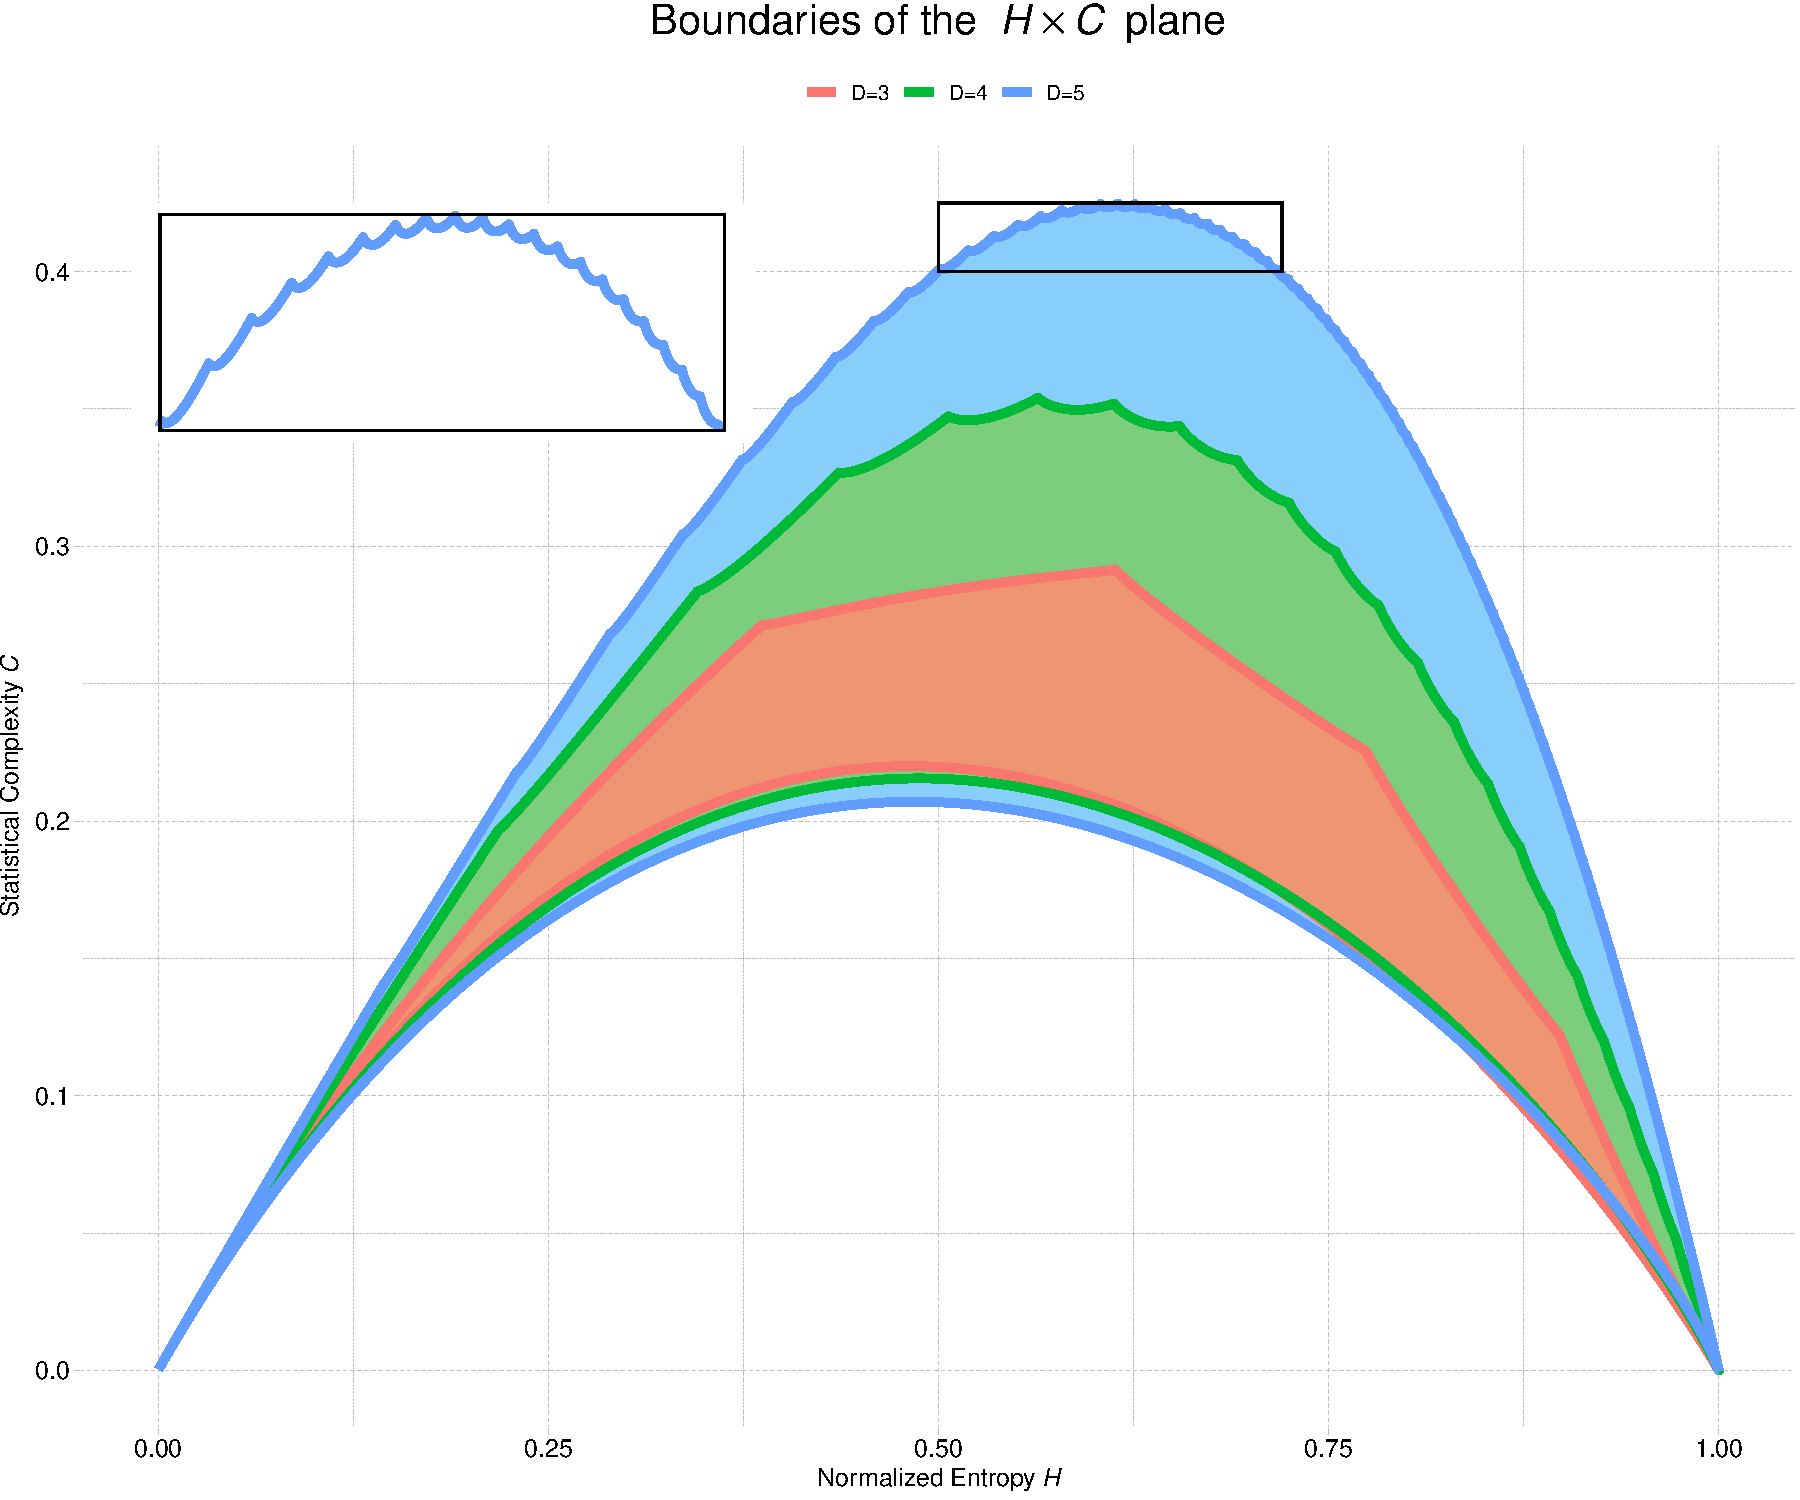
\includegraphics[width=\linewidth]{Figures/BoundariesPlot}
    \caption{Boundaries of the $H\times C$ plane for $D=3,4,5$.}\label{fig:Boundaries}
\end{figure}

We illustrate the use of the Complexity-Entropy ($H\times C$) with the following time series:
\begin{itemize}
    \item \textbf{$f^{-k}$ noises}. Correspond to colored noise sequences generated synthetically using the power spectrum $f^{-k}$~\citep{DistinguishingNoiseFromChaos}.
    Here, we opt to use the following configurations of the spectrum: white ($k=0$), $k=-1/2$, pink ($k=1$), $k=3/2$, red ($k=2$), $=5/2$, and $k=3$;
    \item \textbf{Logistic maps}. The classical chaotic map defined by the formula $x_t = r x_{t-1} (1 - x_{t-1})$~\citep{peitgen2006chaos}.
    In this work, we use this chaotic logistic series with the parameters $r = 3.6$ and $4$;
    \item \textbf{Deterministic series}. Monotonic increasing ($\log(x_t+0.1)$, $x_t=\{1,2,\dots,10^4$) and periodic ($\sin(2x_t)\cos(2x_t)$, with $0\leq x_t\leq 2\pi$ over ten thousand equally spaced points).
\end{itemize}
In all cases, we used $D=6$ and $\tau=1$.
Fig.~\ref{fig:Histograms} shows nine of the histograms produced by these series using the Mersenne-Twister pseudorandom number generator;
we omitted those corresponding to the deterministic series, as they produce one and two nonzero bins.
As we can see, as we add more correlation structures, $f^{-k}$ noises have a less uniform histogram, making it more evident that some ordinal patterns stand out and are more frequent than others.
Therefore, we have an indication that there is a structure of dependence between such elements, making them more deterministic.

\begin{figure}
    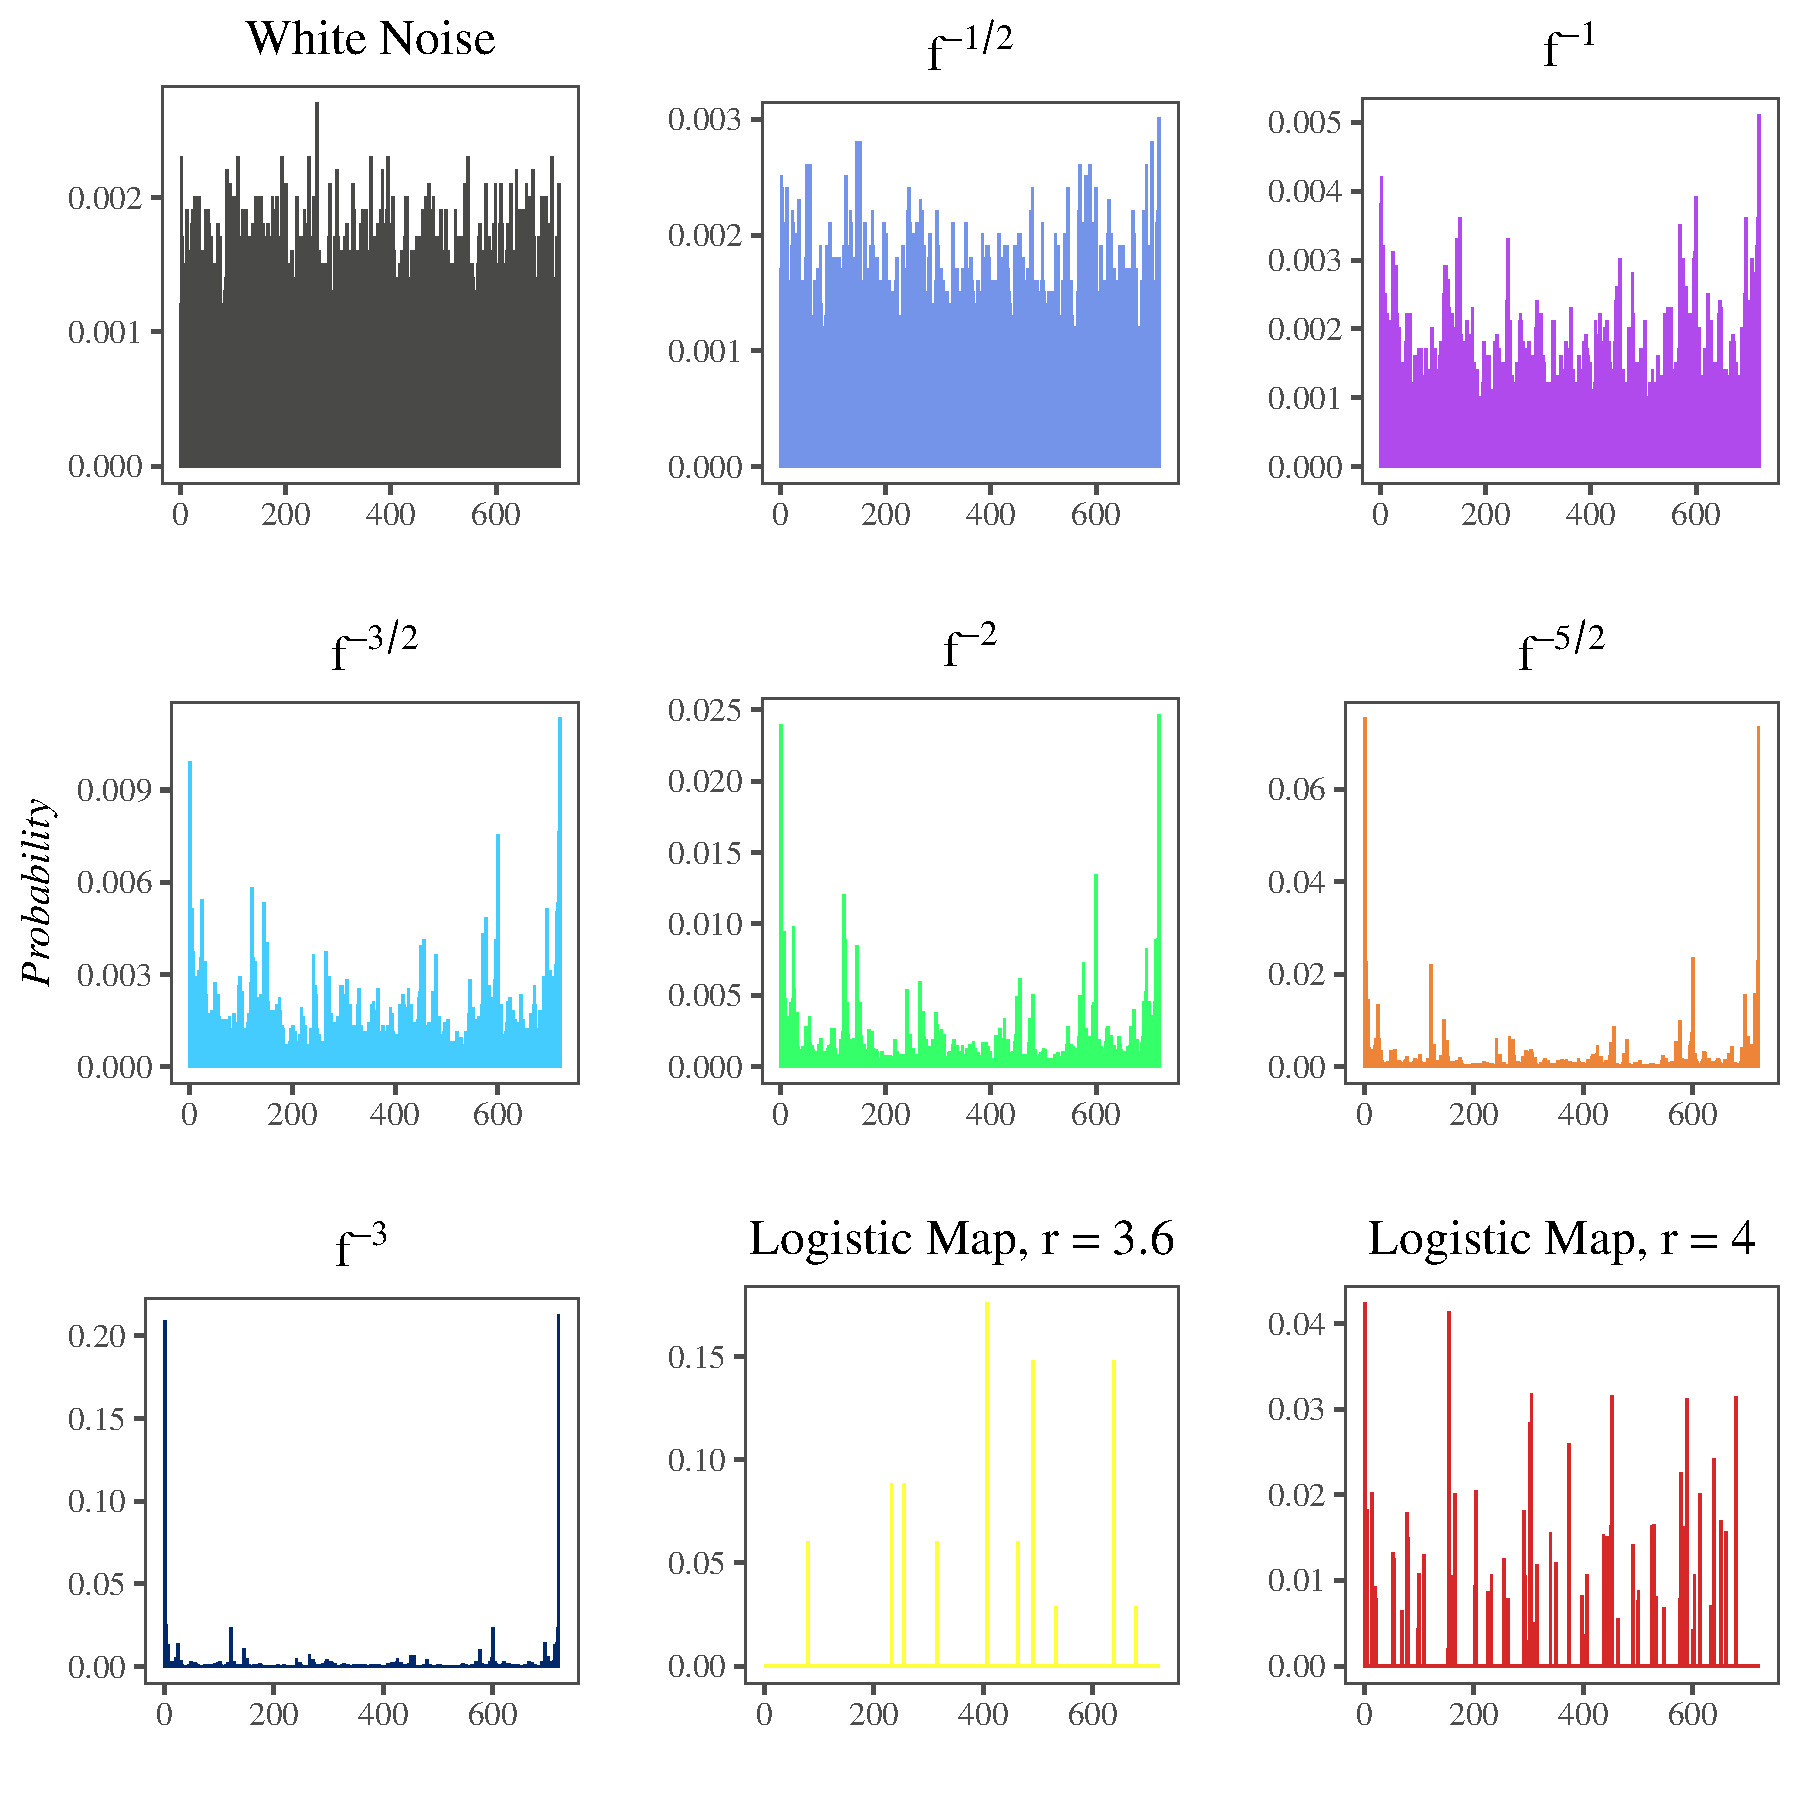
\includegraphics[width=\linewidth]{Figures/h.pdf}
	\caption{Patterns histograms of selected time series with $D=6$, $\tau=1$ and $T = \num[scientific-notation=true]{e4}$.}
	\label{fig:Histograms}
\end{figure}

Fig.~\ref{fig:AllSystems} shows the $H\times C$ plane with the bounds for $D=6$, the time series, and the points they were mapped onto.
The points due to $f^{-k}$ noises appear joined by dotted segments.
It is noticeable that deterministic patterns have more complexity than random ones.
Also, points related to $f^{-k}$ noises tend to clutter for $k<1$, having the highest entropy values.

\begin{figure}
    \centering
    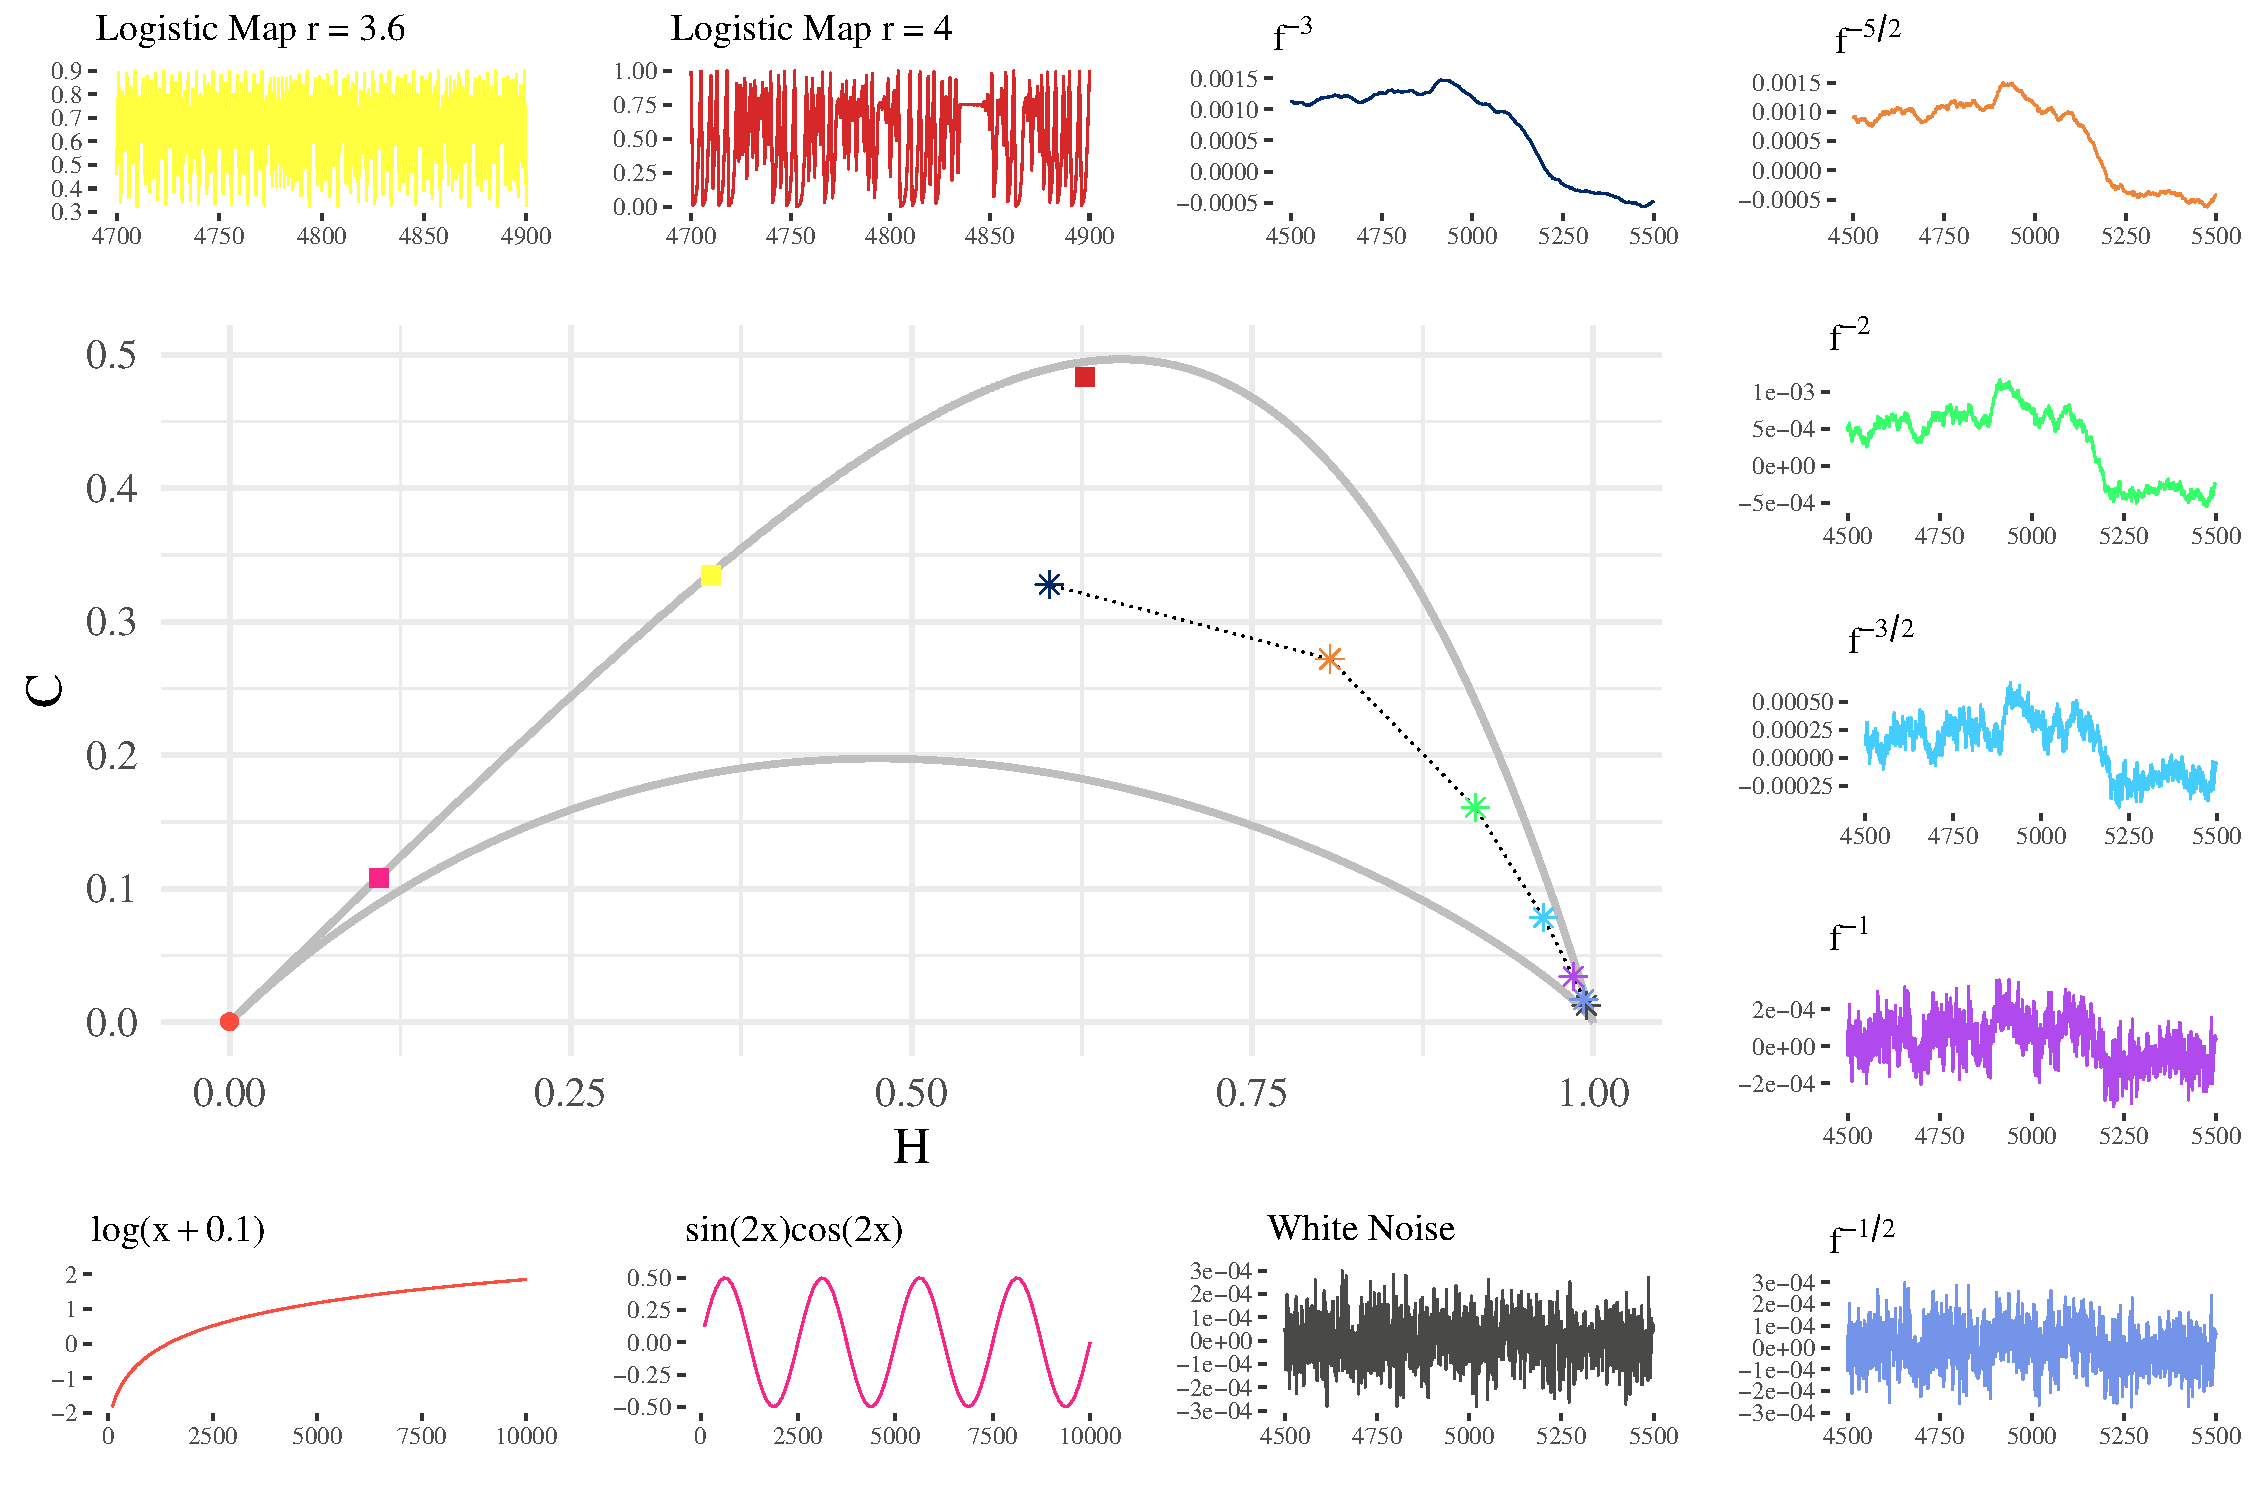
\includegraphics[width=\linewidth]{Figures/AllSystems.pdf}
    \caption{Eleven systems and their points in the $H\times C$ plane when we apply $D = 6$, $\tau = 1$ and $T = \num[scientific-notation=true]{e4}$.}
    \label{fig:AllSystems}
\end{figure}

	

